%%%%%%%%%%%%%%%%%%%%%%%%%%%%%%%%%%%%%%%%%
% Jacobs Landscape Poster
% LaTeX Template
% Version 1.0 (29/03/13)
%
% Created by:
% Computational Physics and Biophysics Group, Jacobs University
% https://teamwork.jacobs-university.de:8443/confluence/display/CoPandBiG/LaTeX+Poster
% 
% Further modified by:
% Nathaniel Johnston (nathaniel@njohnston.ca)
%
% This template has been downloaded from:
% http://www.LaTeXTemplates.com
%
% 
% Masaryk University presentation themes were downloaded from:
% https://www.overleaf.com/gallery/tagged/muni
%
% and ported into Jacobs Landscape Poster by:
% Jumaidil Awal (ideal1st.here@googlemail.com)
% 
% Jacobs Landscape Poster License:
% CC BY-NC-SA 3.0 (http://creativecommons.org/licenses/by-nc-sa/3.0/)
%
% Masaryk University's fibeamer theme license:
% Copyright 2015  Vít Novotný <witiko@mail.muni.cz>
% Faculty of Informatics, Masaryk University (Brno, Czech Republic)
% under Latex Project Public License
%
%%%%%%%%%%%%%%%%%%%%%%%%%%%%%%%%%%%%%%%%%

%----------------------------------------------------------------------------------------
%	PACKAGES AND OTHER DOCUMENT CONFIGURATIONS
%----------------------------------------------------------------------------------------

\documentclass[final]{beamer}

\usepackage[scale=1.15,size=custom, width=106,height=92]{beamerposter} % Use the beamerposter package for laying out the poster

\newlength{\sepwid}
\newlength{\onecolwid}
\newlength{\twocolwid}
\newlength{\threecolwid}


% \usetheme{confposter} % Use the confposter theme supplied with this template
\usetheme[faculty=chemo]{fibeamer} % Uncomment to use Masaryk University's fibeamer theme instead.


%-----------------------------------------------------------
% Define the column widths and overall poster size
% To set effective sepwid, onecolwid and twocolwid values, first choose how many columns you want and how much separation you want between columns
% In this template, the separation width chosen is 0.024 of the paper width and a 4-column layout
% onecolwid should therefore be (1-(# of columns+1)*sepwid)/# of columns e.g. (1-(4+1)*0.024)/4 = 0.22
% Set twocolwid to be (2*onecolwid)+sepwid = 0.464
% Set threecolwid to be (3*onecolwid)+2*sepwid = 0.708


%-----------------------------------------------------------

\usepackage{graphicx}  % Required for including images

\usepackage{booktabs} % Top and bottom rules for tables

%----------------------------------------------------------------------------------------
%	TITLE SECTION 
%----------------------------------------------------------------------------------------

\title{EPIC Dashboard: A modular and extendable approach to disaster data analytics} % Poster title

\author{Gerard Casas Saez, Prof. Kenneth M. Anderson} % Author(s)

\institute{University of Colorado Boulder, Department of Computer Science} % Institution(s)

%----------------------------------------------------------------------------------------

\begin{document}
\setlength{\paperwidth}{106cm} % A0 width: 46.8in
\setlength{\paperheight}{92cm} % A0 height: 33.1in
%\setbeamercolor{block title}{fg=ngreen,bg=white} % Colors of the block titles
%\setbeamercolor{block body}{fg=black,bg=white} % Colors of the body of blocks
%\setbeamercolor{block alerted title}{fg=white,bg=dblue!70} % Colors of the highlighted block titles
%\setbeamercolor{block alerted body}{fg=black,bg=dblue!10} % Colors of the body of highlighted blocks
% Many more colors are available for use in beamerthemeconfposter.sty
\setlength{\sepwid}{0.024\paperwidth} % Separation width (white space) between columns
\setlength{\onecolwid}{0.21\paperwidth} % Width of one column
\setlength{\twocolwid}{0.451\paperwidth} % Width of two columns
\setlength{\threecolwid}{0.678\paperwidth} % Width of three columns
% \setlength{\topmargin}{-8cm} % Reduce the top margin size
\addtobeamertemplate{block end}{}{\vspace*{2ex}} % White space under blocks
\addtobeamertemplate{block example end}{}{\vspace*{2ex}} % White space under example blocks
\addtobeamertemplate{block alerted end}{}{\vspace*{2ex}} % White space under highlighted (alert) blocks

\setlength{\belowcaptionskip}{2ex} % White space under figures
\setlength\belowdisplayshortskip{2ex} % White space under equations
\begin{darkframes} % Uncomment for dark theme, don't forget to \end{darkframes}
\begin{frame} % The whole poster is enclosed in one beamer frame

%==========================Begin Head===============================

  \begin{columns}
  \begin{column}{\linewidth}
    \vskip0.1cm
    \centering
    \usebeamercolor{title in headline}{\color{fg}\Huge{\textbf{\inserttitle}}\\[0.5ex]}
    \usebeamercolor{author in headline}{\color{fg}\Large{\insertauthor}\\[1ex]}
    \usebeamercolor{institute in headline}{\color{fg}\large{\insertinstitute}\\[1ex]}
    \vskip1cm
  \end{column}
  \vspace{1cm}
  \end{columns}
 \vspace{1cm}

%==========================End Head===============================

\begin{columns}[t] % The whole poster consists of three major columns, the second of which is split into two columns twice - the [t] option aligns each column's content to the top

\begin{column}{\sepwid}\end{column} % Empty spacer column

\begin{column}{\onecolwid} % The first column

%----------------------------------------------------------------------------------------
%	OBJECTIVES
%----------------------------------------------------------------------------------------

% \begin{exampleblock}{Abstract}

% The field of adversarial machine learning is also useful for identification of vulnerabilities in a machine learning approach in presence of adversarial settings
% \begin{itemize}
% \item Illustrate the design cycle of a learning-based pattern recognition system for adversarial tasks.
% \item Performance of pattern classifiers and deep learning algorithms under attack, evaluate their vulnerabilities.
% \item Pattern recognition tasks like object recognition in images, biometric identity recognition, spam and malware detection.
% \end{itemize}

% \end{exampleblock}

%----------------------------------------------------------------------------------------
%	INTRODUCTION
%----------------------------------------------------------------------------------------

\begin{exampleblock}{Introduction}
\textbf{Big Data Analytics} is a research area undergoing intense interest and rapid development. Data is being generated by sensors and computing systems at an ever-increasing rate. Indeed, it is estimated that every month, seventy-two petabytes of
information are moved around the Internet. This amount is expected to grow
to \textbf{232 petabytes/month by 2021}. 

Thanks to the popularization of \textbf{managed cloud computing services}, many big data tools have become easier to use. \textbf{Managed SQL engines for large non-structured datasets} are an example as they allow us to perform OLAP queries without having to support large and complex infrastructure designs. Thanks to all this we can start to head back to the pre-NoSQL query types without the maintenance issues of NoSQL infrastructure.
\end{exampleblock}
\begin{exampleblock}{Motivation}
At Project EPIC most work has been based on 2 monolith apps: \textbf{EPIC Collect}\cite{schram2012mysql} and \textbf{EPIC Analyze}\cite{anderson2015design}. Due to recent issues with campus hosting service and lack of maintenance, these apps went offline. The lack of knowledge about the systems made it difficult to fully recover. The data was saved, but the collecting and analysis software was not.

At the same time, various students have struggled to add new features as the app complexity grew. This was mainly due to the monolith nature of the apps. As the codebase extended, more dependencies make it difficult to manage and increased the learning curve for new developers.

The proposed infrastructure for EPIC Dashboard is fully based on \textbf{microservices} to increase modularity between different features and to make it easier to extend. 
\end{exampleblock}
%------------------------------------------------



%----------------------------------------------------------------------------------------

\end{column} % End of the first column

\begin{column}{\sepwid}\end{column} % Empty spacer column

\begin{column}{\twocolwid} % Begin a column which is two columns wide (column 2)

\begin{columns}[t,totalwidth=\twocolwid] % Split up the two columns wide column

\begin{column}{\onecolwid}\vspace{-.74in} % The first column within column 2 (column 2.1)

%----------------------------------------------------------------------------------------
%	MATERIALS
%----------------------------------------------------------------------------------------

\begin{exampleblock}{Data Collection}

Data collection needs to be a reliable pipeline that retrieves, classifies and stores the data we need. In order to make it simpler, Events API abstraction is provided. This service is in charge of triggering changes in a container orchestrated system to collect the data needed accordingly. For reliability, the system is separated into 2 steps ( \textbf{retrieval} and \textbf{classification}) and connected with a \textbf{message queue system}.

\end{exampleblock}
\begin{exampleblock}{Data exploration}

EPIC Dashboard allows for exploration and filtering of datasets. Filtering relies on \textbf{Google BigQuery} database engine, which is a SQL engine for non-structured data. For complex tasks Spark is used. To simplify dataset tagging and exploration the system allows individual tweet annotation, matching the requirement discovered during the development of EPIC Analyze. \cite{anderson2015design}

\end{exampleblock}
%----------------------------------------------------------------------------------------

\end{column} % End of column 2.1
\begin{column}{\sepwid}\end{column} % Empty spacer column

\begin{column}{\onecolwid}\vspace{-.74in} % The second column within column 2 (column 2.2)

%----------------------------------------------------------------------------------------
%	METHODS
%----------------------------------------------------------------------------------------

\begin{exampleblock}{User Interface}

\begin{enumerate}
\item \textbf{Event creation}: An interface that interacts with Events API to create/start/stop events. Triggers changes in collection infrastructure.
\begin{figure}
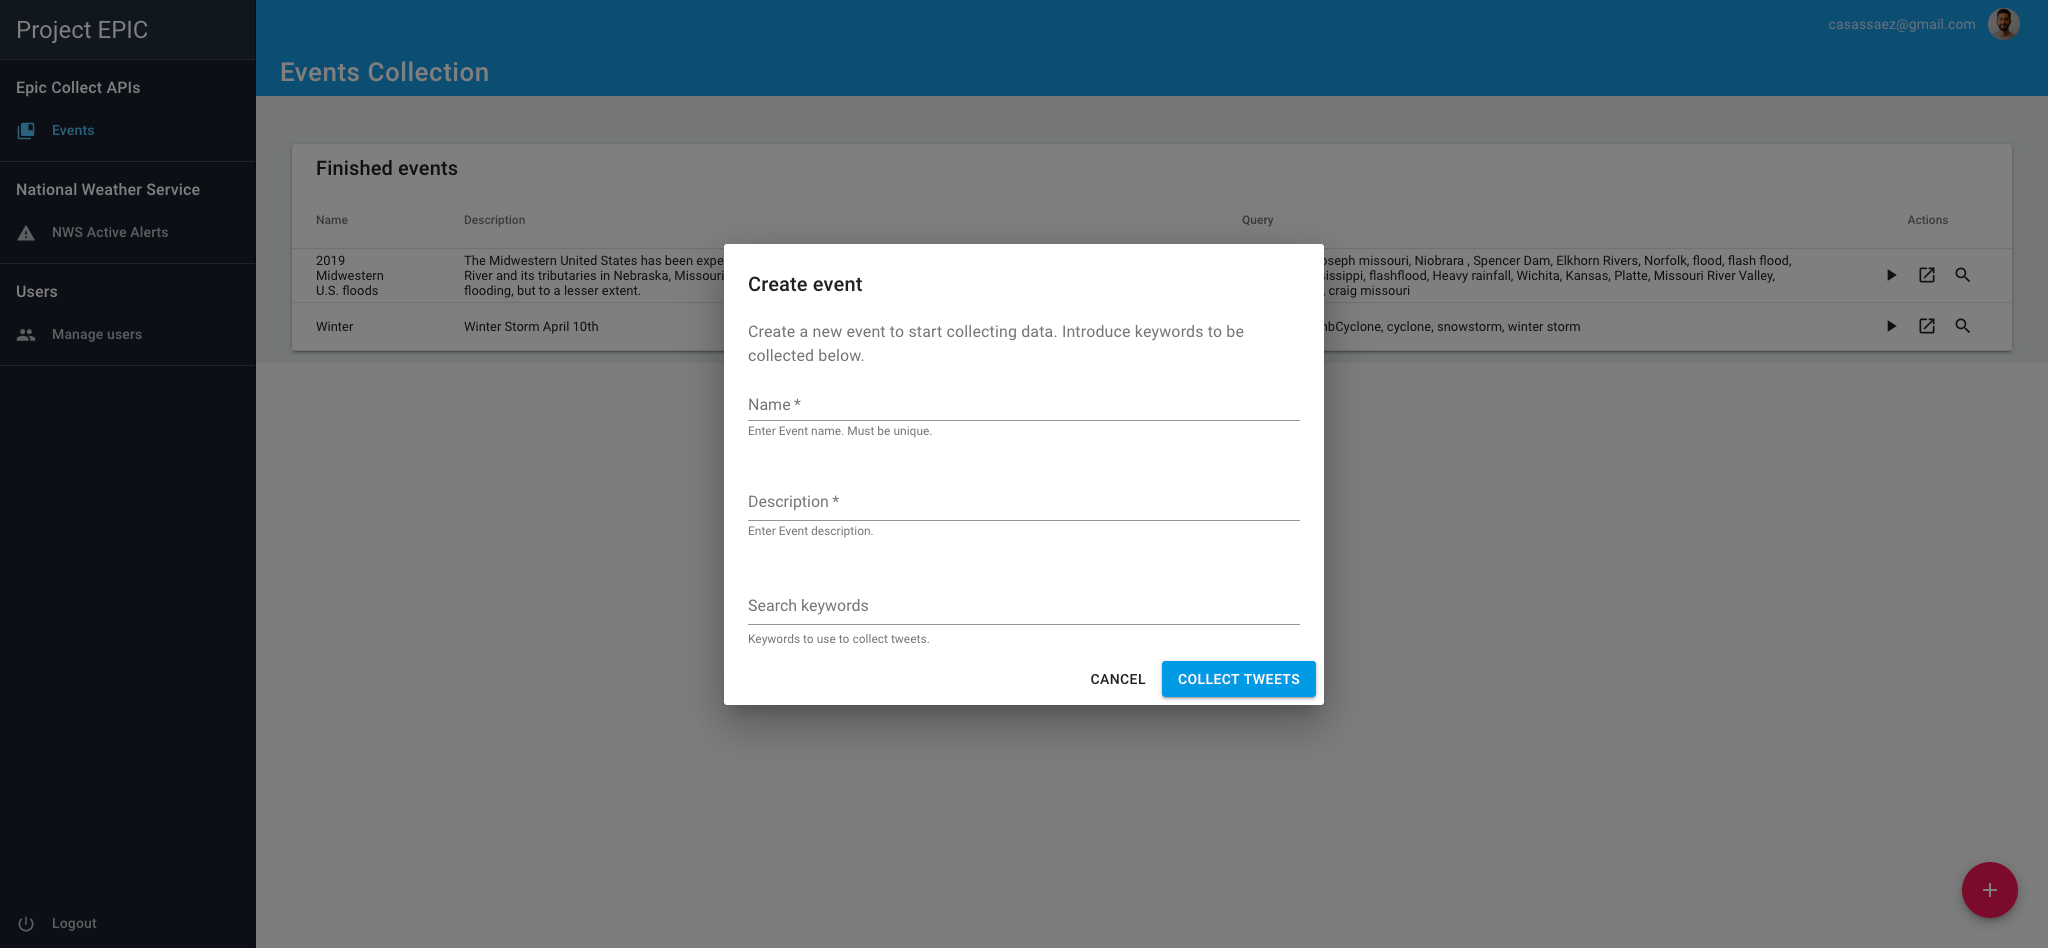
\includegraphics[width=1\linewidth]{img/event_creating.png}
\end{figure}
\item \textbf{Tweet tagging}: Dataset exploration and annotation interface. Allows analysts to add tags to individual tweets.
\begin{figure}
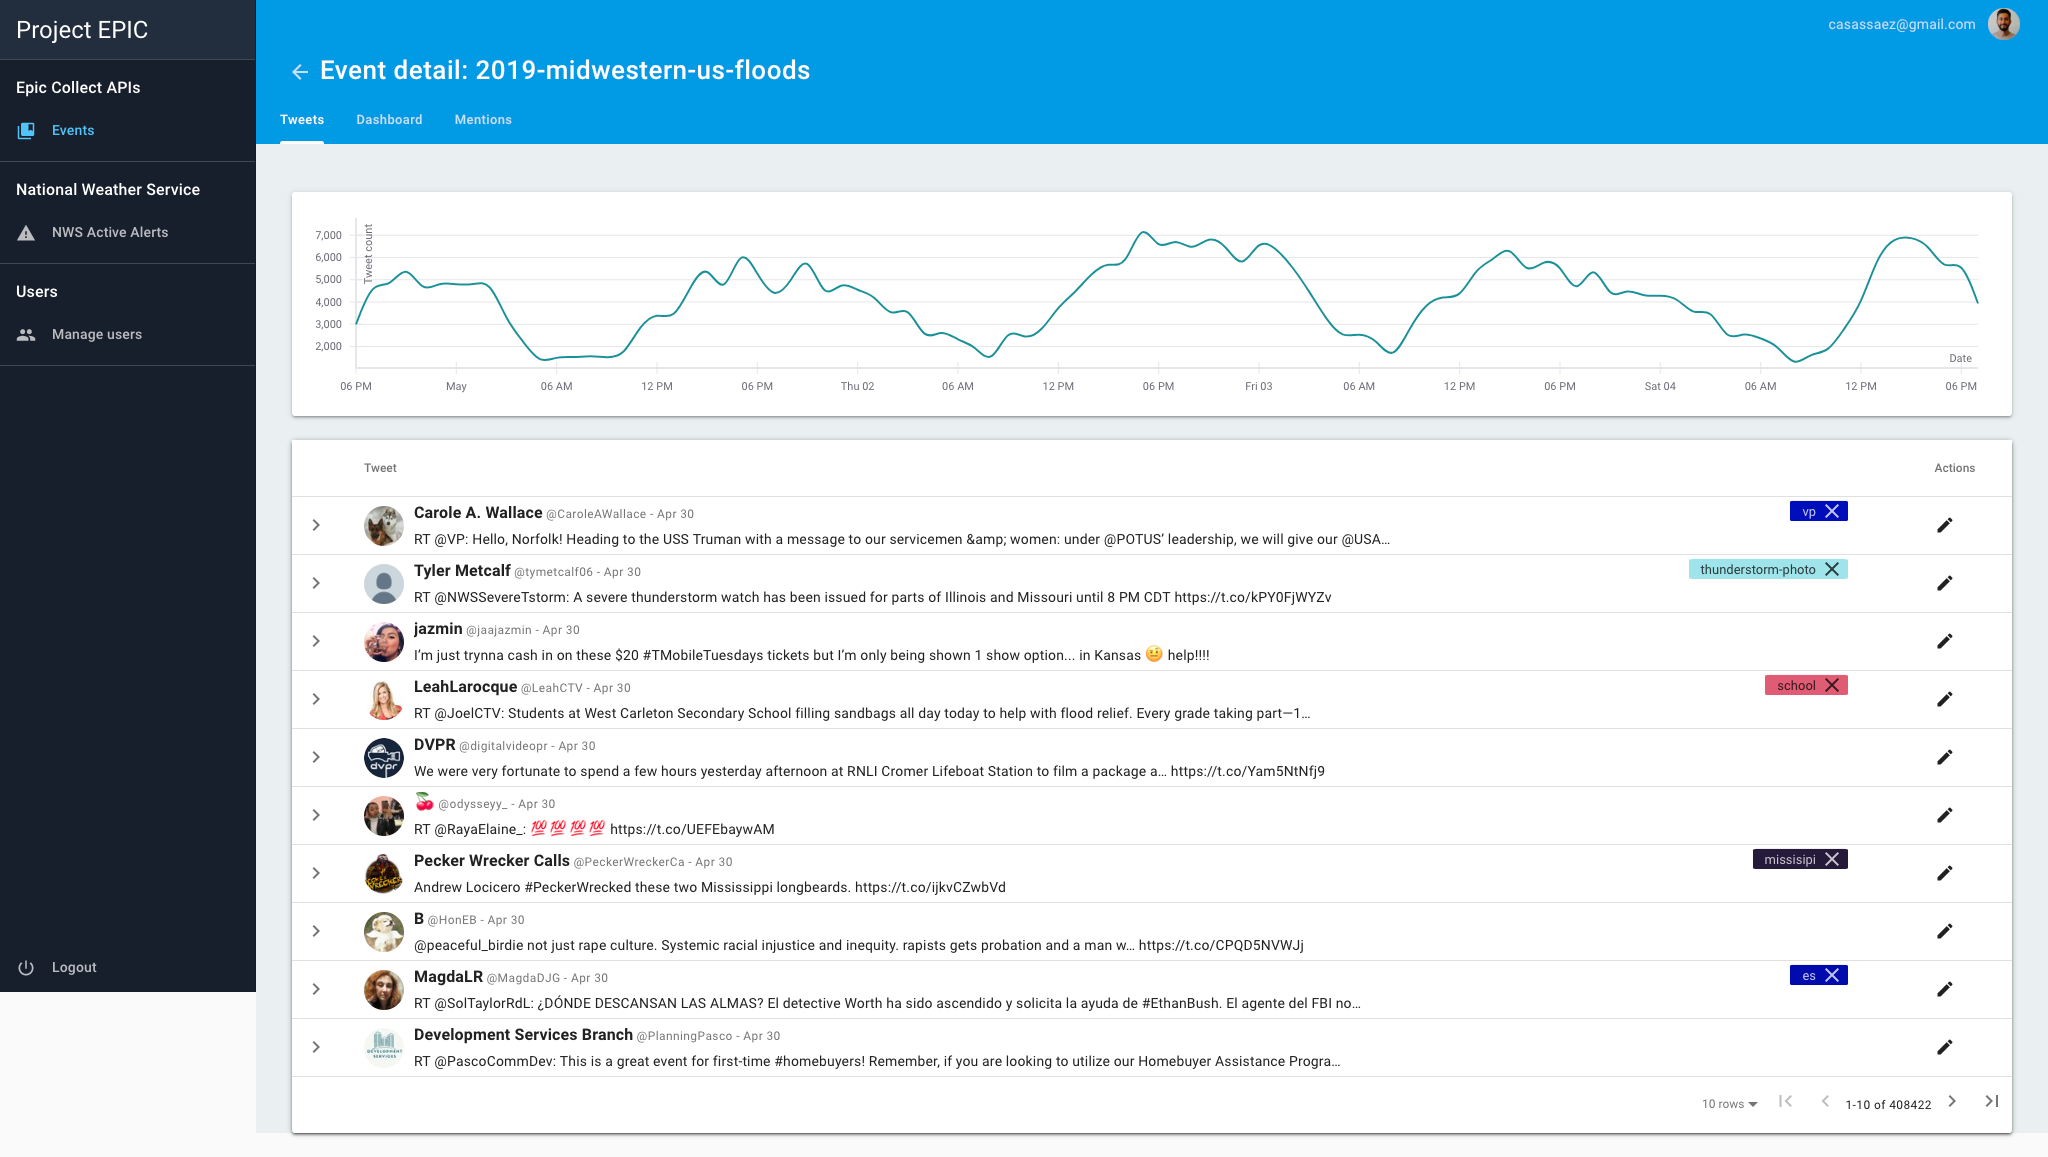
\includegraphics[width=1\linewidth]{img/tweets_tagging.png}
\end{figure}
\end{enumerate}




\end{exampleblock}

%----------------------------------------------------------------------------------------

\end{column} % End of column 2.2

\end{columns} % End of the split of column 2 - any content after this will now take up 2 columns width

%----------------------------------------------------------------------------------------
%	IMPORTANT RESULT
%----------------------------------------------------------------------------------------

\begin{alertblock}{Infrastructure diagram}
\begin{figure}
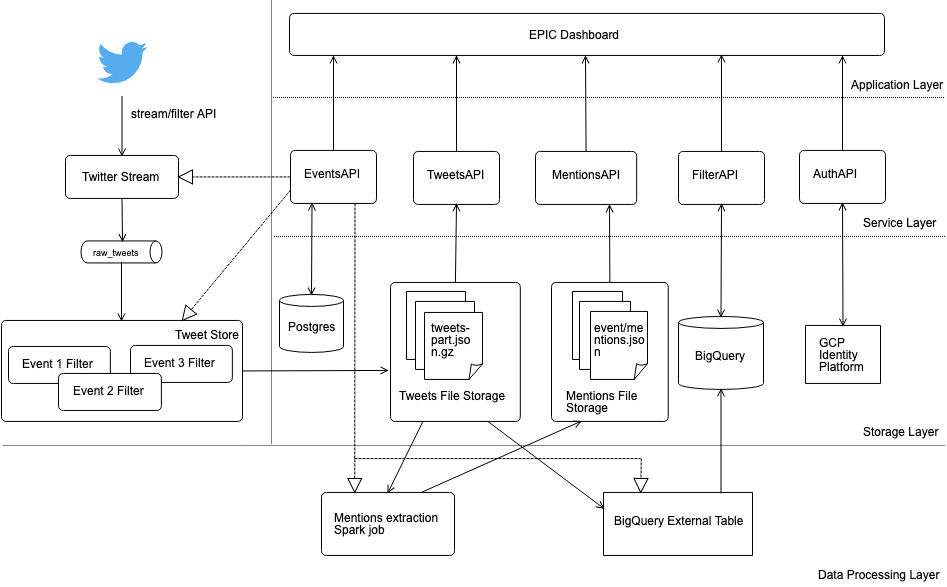
\includegraphics[width=1\twocolwid]{img/infra_white.png}
\end{figure}

\end{alertblock} 

%----------------------------------------------------------------------------------------

\begin{columns}[t,totalwidth=\twocolwid] % Split up the two columns wide column again

\begin{column}{\onecolwid} % The first column within column 2 (column 2.1)

%----------------------------------------------------------------------------------------
%	MATHEMATICAL SECTION
%----------------------------------------------------------------------------------------



%----------------------------------------------------------------------------------------

\end{column} % End of column 2.1
\begin{column}{\sepwid}\end{column} % Empty spacer column

\begin{column}{\onecolwid} % The second column within column 2 (column 2.2)

%----------------------------------------------------------------------------------------
%	RESULTS
%----------------------------------------------------------------------------------------

% \begin{exampleblock}{Results}

% \begin{figure}
% \includegraphics[width=0.8\linewidth]{img/placeholder.jpg}
% \caption{Figure caption}
% \end{figure}

% Nunc tempus venenatis facilisis. Curabitur suscipit consequat eros non porttitor. Sed a massa dolor, id ornare enim:

% \begin{table}
% \vspace{2ex}
% \begin{tabular}{l l l}
% \toprule
% \textbf{Treatments} & \textbf{Response 1} & \textbf{Response 2}\\
% \midrule
% Treatment 1 & 0.0003262 & 0.562 \\
% Treatment 2 & 0.0015681 & 0.910 \\
% Treatment 3 & 0.0009271 & 0.296 \\
% \bottomrule
% \end{tabular}
% \caption{Table caption}
% \end{table}

% \end{exampleblock}

%----------------------------------------------------------------------------------------

\end{column} % End of column 2.2

\end{columns} % End of the split of column 2

\end{column} % End of the second column

\begin{column}{\sepwid}\end{column} % Empty spacer column

\begin{column}{\onecolwid} % The third column

%----------------------------------------------------------------------------------------
%	CONCLUSION
%----------------------------------------------------------------------------------------

\begin{exampleblock}{Results}

 EPIC Dashboard infrastructure replicates most of EPIC Collect and EPIC Analyze existing features while splitting the code into smaller units (microservices) on a hybrid cloud architecture. This approach improves on:
 
 \begin{itemize}
     \item \textbf{Reliability}: Managed cloud services have contracts that specify the required reliability and availability.
     \item \textbf{Extensibility}: New developers can extend the functionality of the system by adding new services on top of the existing data, without needing to learn how the full system works.
     \item \textbf{Modularity}: Components can be fully replaced and updated individually. This allows keeping component updated with new offerings from the industry.
 \end{itemize}


Cloud Computing is democratizing access to Big Data Analytics systems. Thanks to container orchestrated systems, we can make hybrid like infrastructures that reuse existing analytics software and allow us to leverage the power of cloud tools. 

\end{exampleblock}

%----------------------------------------------------------------------------------------
%	REFERENCES
%----------------------------------------------------------------------------------------

\begin{exampleblock}{References}

 % Insert publications even if they are not cited in the poster
\small{\bibliographystyle{unsrt}
\bibliography{sample}\vspace{1cm}}
\end{exampleblock}

%----------------------------------------------------------------------------------------
%	ACKNOWLEDGEMENTS
%----------------------------------------------------------------------------------------

%\setbeamercolor{block title}{fg=red,bg=white} % Change the block title color

%\begin{exampleblock}{Acknowledgements}

%\small{\rmfamily{Nam mollis tristique neque eu luctus. Suspendisse rutrum congue nisi sed convallis. Aenean id neque dolor. Pellentesque habitant morbi tristique senectus et netus et malesuada fames ac turpis egestas.}} \\

%\end{exampleblock}

%----------------------------------------------------------------------------------------
%	CONTACT INFORMATION
%----------------------------------------------------------------------------------------

%\setbeamercolor{block alerted title}{fg=black,bg=norange} % Change the alert block title colors
%\setbeamercolor{block alerted body}{fg=black,bg=white} % Change the alert block body colors

\begin{block}{Contact Information}

\begin{itemize}
\item Web: \href{http://epic.cs.colorado.edu/}{http://epic.cs.colorado.edu/}
\item Email: \href{mailto:geca5834@colorado.edu}{geca5834@colorado.edu}
\end{itemize}

\end{block}

% \begin{tabular}{rr}
% \hspace{0.3\linewidth} & \includegraphics[width=0.5\linewidth]{img/logo.png}
% \end{tabular}

%----------------------------------------------------------------------------------------

\end{column} % End of the third column

\begin{column}{\sepwid}\end{column} % Empty spacer column

\end{columns} % End of all the columns in the poster

\end{frame} % End of the enclosing frame
\end{darkframes} % Uncomment for dark theme
\end{document}
